\subsubsection{Utilizzo di ANTLR nella repository \textit{unina-Basalt}}
Come già detto in precedenza, per la repository \textit{unina-Basalt} è stato utilizzato ANTLR4
come frontend framework. Tale scelta implica l'utilizzo di un parser autogenerato. \\

In particolare, lo strumento da riga di comando \texttt{antlr4} è stato utilizzato per generare 
il codice sorgente della classe \texttt{BasaltParserVisitor}, il quale estende 
\texttt{AbstractParseTreeVisitor}. \\

La classe \texttt{BasaltParserVisitor} è stata pensata dagli sviluppatori di 
ANTLR per essere estesa da una implementazione concreta. Tale classe infatti 
espone dei metodi astratti che devono essere implementati per poter
effettuare il parsing del codice sorgente. \\

Nel caso specifico di Basalt, la classe \texttt{BasaltParserVisitor} è stata
estesa dalla classe \texttt{ConcreteBasaltParserVisitor}, la quale implementa i 
suddetti metodi astratti. \\

\begin{figure}[H]
    \centering
        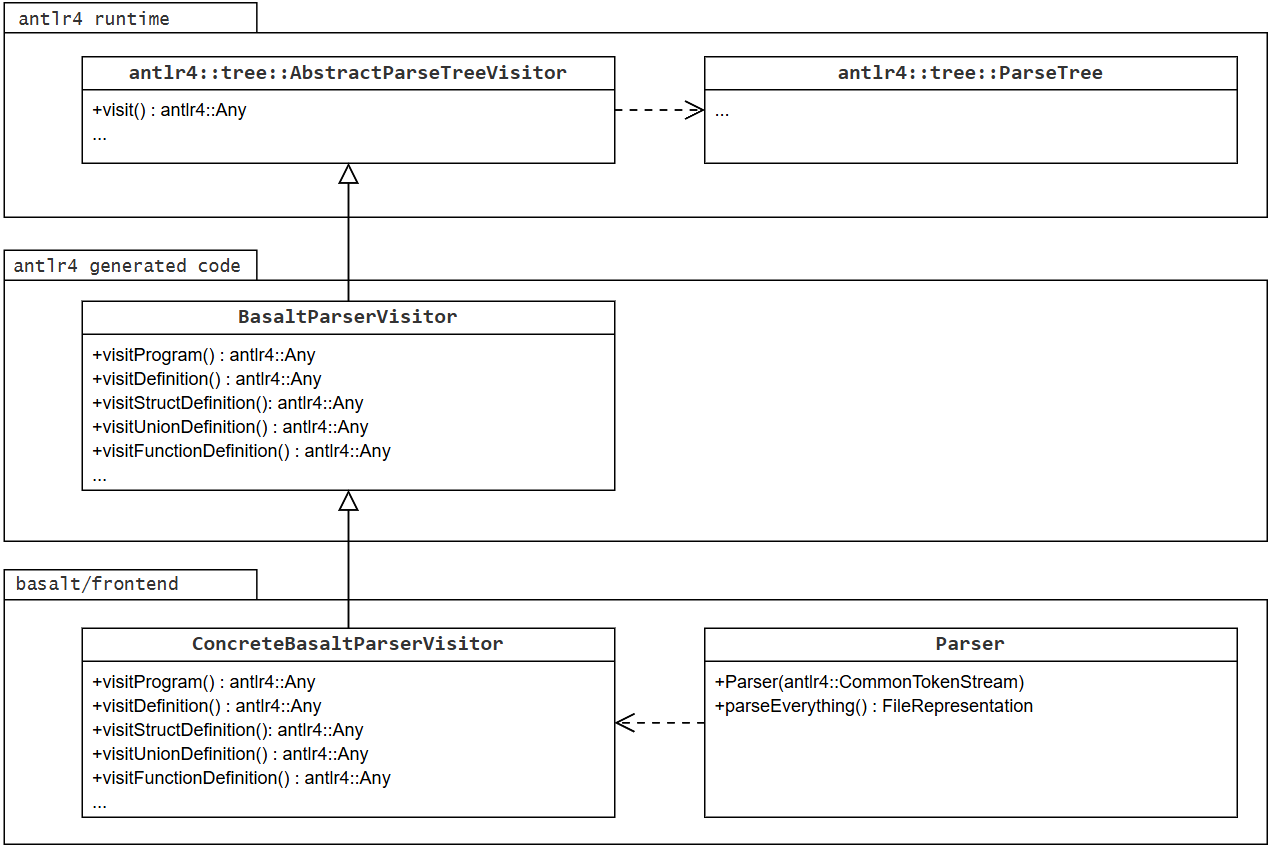
\includegraphics[width=1\textwidth]{../../Assets/ANTLR-PARSER-UML.png} 
    \caption{UML-Class-diagram del parser con ANTLR4}
\end{figure}

\newpage

Il risultato di ogni chiamata ai vari metodi di \texttt{ConcreteBasaltParserVisitor} è
un oggetto di tipo \texttt{antlr4::Any}, il è un tipo di dato fornito da ANTLR per 
modellare il risultato di una generica visita al parse tree. \\

Nel caso specifico, il risultato di ogni metodo di \texttt{ConcreteBasaltParserVisitor}
è un'istanza di una classe definita nella codebase di Basalt, la quale rappresenta
un'entità del linguaggio. \\

Utilizzando il metodo \texttt{parseProgram} il risultato sarà un'istanza di 
\texttt{FileRepresentation}, il quale codifica l'intero contenuto di un file sorgente. \\

Come input del costruttore della classe \texttt{Parser}, la quale è un wrapper 
su \texttt{ConcreteBasaltParserVisitor}, viene passato un oggetto di tipo
\texttt{antlr4::CommonTokenStream}, il quale rappresenta il contenuto di un file sorgente. \\

Per ottenere un oggetto di tipo \texttt{antlr4::CommonTokenStream} è necessario
utilizzare la classe \texttt{Tokenizer}, la quale è a sua volta un wrapper sulla classe 
autogenerata \texttt{BasaltLexer} (l'utilizzo dei wrapper serve ad esporre la stessa API
della repository principale, e consentire una migliore integrazione tra le due). \\

\begin{figure}[H]
    \centering
        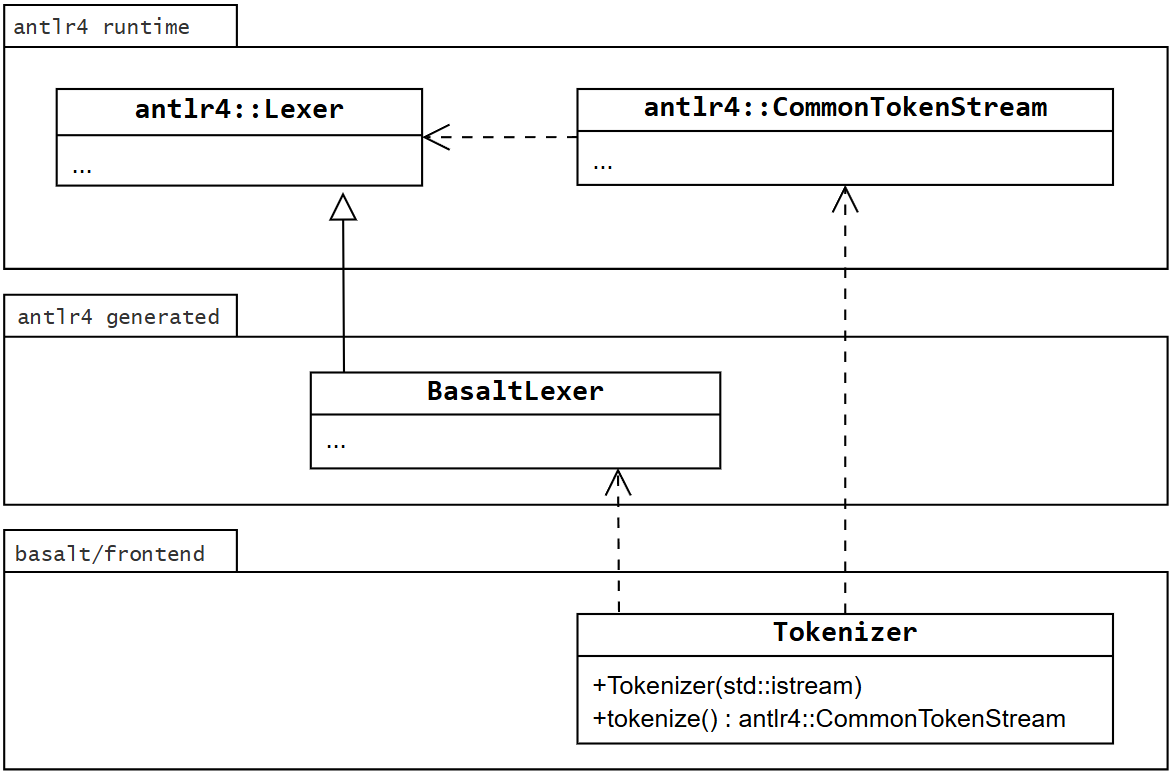
\includegraphics[width=1\textwidth]{../../Assets/ANTLR-TOKENIZER-UML.png} 
    \caption{UML-Class-diagram del parser con ANTLR4}
\end{figure}